\chapter{Probability Theory}\label{chapter:probability}

    The majority of this chapter uses the language of measure theory. See \cref{chapter:measure} for an introduction. The section on optimal transport is partially based on~\citet{beiglboeck_general_2009,nenna_monge_2020}.

    \minitoc

\section{Probability}

    The Kolmogorov axioms of probability state when a set admits the definition of a probability theory.
    \begin{axiom}[Kolmogorov]\index{Kolmogorov!axioms}\index{probability!space}\index{sample!space}\label{prob:kolmogorov_axioms}
        A \textbf{probability space} $(\Omega,\Sigma,P)$ is a measure space (\cref{measure:measure_space}) with normalized measure $P(X)=1$. The set $\Omega$ is called the \textbf{sample space}.
    \end{axiom}

    \newdef{Random variable}{\index{random!variable}
        A measurable function $X:\Omega\rightarrow\mathbb{R}$ on a probability space  $(\Omega,\Sigma,P)$, i.e.
        \begin{gather}
            \forall a\in\mathbb{R}:X^{-1}\bigl([a,+\infty[\bigr)=\{\omega\in\Omega\mid X(\omega)\geq a\}\in\Sigma\,.
        \end{gather}
    }

    \newdef{$\sigma$-algebra of a random variable}{\index{$\sigma$!algebra}
        Let $X$ be a random variable defined on $(\Omega,\Sigma,P)$ and denote the Borel $\sigma$-algebra of $\mathbb{R}$ by $\mathcal{B}$. The following collection of sets is a $\sigma$-algebra:
        \begin{gather}
            \label{prob:sigma_algebra_generated_random_variable}
            X^{-1}(\mathcal{B}) := \{S\in\Sigma\mid\exists B\in\mathcal{B}:S = X^{-1}(B)\}\,.
        \end{gather}
    }
    \begin{notation}
        The $\sigma$-algebra generated by the random variable $X$ is often denoted by $\mathcal{F}\!\!_X$ instead of \cref{set:notation:generated_sigma_algebra}.
    \end{notation}

    \newdef{Event}{\index{event}
        Let $(\Omega,\Sigma,P)$ be a probability space. An element $S$ of the $\sigma$-algebra $\Sigma$ is called an event.

        From this definition, it is clear that a single possible outcome of a measurement can be part of multiple events. So, although only one outcome can occur at the same time, multiple events can occur simultaneously.
    }
    \begin{remark*}
        The Kolmogorov axioms use the $\sigma$-algebra (\cref{set:sigma_algebra}) of events instead of the power set (\cref{set:power_set}) of all events. Intuitively this seems to mean that some possible outcomes are not treated as events. However, one can make sure that the $\sigma$-algebra still contains all `useful' events by using a `nice' definition of probability spaces.
    \end{remark*}

    \newdef{Disjoint events}{\index{disjoint}
        Two events $A$ and $B$ are said to be disjoint if they cannot happen at the same time:
        \begin{gather}
            P(A\cap B) = 0\,.
        \end{gather}
    }

    The finite additivity of measures implies the following rules.
    \newformula{Union}{\label{prob:union}
        Let $A,B$ be two events. The probability that at least one of them occurs is given by the following formula:
        \begin{gather}
            P(A\cup B) = P(A) + P(B) - P(A\cap B)\,.
        \end{gather}
    }
    \newformula{Complement}{\index{complement}\label{prob:complement}
        Let $A$ be an event. The probability of $A$ being false is denoted as $P\bigl(\overline{A}\bigr)$ and is given by
        \begin{gather}
            P\bigl(\overline{A}\bigr) = 1 - P(A)\,.
        \end{gather}
    }
    \begin{result}
        From the previous formula and de Morgan's laws~\eqref{set:de_morgan_union} and~\eqref{set:de_morgan_intersection}, one can derive the following formula:
        \begin{gather}
            P\bigl(\overline{A}\cap\overline{B}\bigr) = 1 - P(A\cup B)\,.
        \end{gather}
    \end{result}

\section{Conditional probability}

    \newdef{Conditional probability}{\index{probability!conditional}\label{prob:conditional_probability}
        Let $A,B$ be two events. The probability of $A$ given that $B$ is true, denoted by $P(A\mid B)$, is defined as follows:
        \begin{gather}
            P(A\mid B) := \frac{P(A\cap B)}{P(B)}\,.
        \end{gather}
    }
    By interchanging $A$ and $B$ in the previous equation and by observing that this has no effect on the quantity $P(A\cap B)$, the following important result can be derived.
    \begin{theorem}[Bayes]\index{Bayes}\label{prob:bayes}
        Let $A,B$ be two events.
        \begin{gather}
            P(A\mid B) = \frac{P(B\mid A)P(A)}{P(B)}
        \end{gather}
    \end{theorem}

    \begin{formula}\label{prob:total_probability_conditional}
        Let $\seq{B}$ be a pairwise disjoint cover of $\Omega$. The total probability of an event $A$ can be calculated as follows:
        \begin{gather}
            P(A) = \sum_{n=0}^{+\infty}P(A\mid B_n)P(B_n)\,.
        \end{gather}
    \end{formula}

    \newdef{Independent events}{\index{independence}
        Let $A,B$ be two events. $A$ and $B$ are said to be independent if they satisfy the following relation:
        \begin{gather}
            P(A\cap B) = P(A)P(B)\,.
        \end{gather}
    }
    \begin{result}
        If $A$ and $B$ are two independent events, Bayes' theorem simplifies to
        \begin{gather}
            P(A\mid B) = P(A)\,.
        \end{gather}
    \end{result}

    The above definition can be generalized to multiple events.
    \begin{definition}[Independent events]\index{independence}
        The events $\{A_1,\ldots,A_n\}$ are said to be independent if, for each choice of $k\leq n$ events, the probability of their intersection is equal to the product of their individual probabilities.
    \end{definition}

    This definition can be stated in terms of $\sigma$-algebras.
    \newdef{Independence}{\index{independence}\label{prob:independent_sigma_algebras}
        The $\sigma$-algebras $\{\mathcal{F}\!_1,\ldots,\mathcal{F}\!\!_n\}$ defined on a probability space $(\Omega,\mathcal{F},P)$ are said to be independent if, for all choices of distinct indices $i_1,\ldots,i_k$ and for all choices of sets $F_{i_n}\in\mathcal{F}\!\!_{i_n}$, the following equation holds:
        \begin{gather}
            P(F_{i_1}\cap\cdots\cap F_{i_k}) = P(F_{i_1})\cdots P(F_{i_k})\,.
        \end{gather}
    }
    \begin{result}
        Two random variables are independent if the $\sigma$-algebras generated by them are independent.
    \end{result}

\section{Probability distributions}\label{section:probability_distributions}
\subsection{Distribution functions}

    \newdef{Probability distribution}{\index{probability!distribution}\label{prob:probability_distribution}
        Let $X$ be a random variable on $(\Omega,\Sigma,P)$. The following function is a probability measure on the Borel $\sigma$-algebra of $\mathbb{R}$:
        \begin{gather}
            P\!_X(B) = P\bigl(X^{-1}(B)\bigr)\,.
        \end{gather}
        This measure is called the probability distribution of $X$.
    }

    \begin{example}[Rademacher variable]\index{Rademacher!variable}\label{prob:rademacher}
        A random variable on $\Omega=\{-1,1\}$ with probability distribution $P\!_X(-1)=P\!_X(1)=\frac{1}{2}$.
    \end{example}

    \newdef{Density}{\index{density}\index{mass}\label{prob:density}
        Consider an integrable function $f\geq0$ and recall \cref{measure:measure_by_integral}. The function $f$ is called the density of the measure $P(A):=\int_Af\,d\lambda$ (with respect to the Lebesgue measure $\lambda$). If the measure is a probability measure, i.e.~it is normalized to 1, $f$ is called a \textbf{probability density function}.

        More generally, by the Radon--Nikodym Theorem~\ref{measure:radon_nikodym}, every absolutely continuous probability distribution $P$ on $\mathbb{R}^n$ is of the form
        \begin{gather}
            P(A) = \Int_Af\,d\lambda
        \end{gather}
        for some integrable function $f$.

        When $P$ is discrete, i.e.~when one works with respect to the counting measure, the Radon--Nikodym derivative is called the \textbf{probability mass function}. (In this compendium, this function will also often be called the density function.)
    }

    \newdef{Cumulative distribution function}{\index{cumulative distribution function}\label{prob:cdf}
        Consider a random variable $X$ and its associated distribution $P\!_X$. The cumulative distribution function $F\!_X:\mathbb{R}\rightarrow[0,1]$ is defined as follows:
        \begin{gather}
            F\!_X(a) := P\!_X\bigl(\{x\in\mathbb{R}\mid x\leq a\}\bigr)\,.
        \end{gather}
    }

    The following is a consequence of the Kolmogorov axioms.
    \begin{result}\label{prob:cdf_axioms}
        Let $F:\mathbb{R}\rightarrow[0,1]$ be a function that satisfies the following three properties:
        \begin{itemize}
            \item $F$ is increasing.
            \item $\ds\lim_{x\rightarrow-\infty}F(x) = 0$ and $\ds\lim_{x\rightarrow\infty}F(x) = 1$.
            \item $F$ is right-continuous, i.e.~$\ds\lim_{y\nearrow y_0}F(y)=F(y_0)$ for all $y_0\in\mathbb{R}$.
        \end{itemize}
        There exists a random variable $X:[0,1]\rightarrow\mathbb{R}$ on the probability space $([0,1],\mathcal{B}_{[0,1]},\lambda_{[0,1]})$, such that $F=F\!_X$, where $\mathcal{B}_{[0,1]}$ is the Borel $\sigma$-algebra of $[0,1]$ with its Euclidean topology.
    \end{result}

    \newdef{Parametric family}{\index{parametric family}
        An indexed family of probability distributions.
    }

    \begin{example}[Mixture family]\index{mixture}
        Consider a collection of distributions $\mathcal{P}\equiv\{P_i\}_{i\leq n}$. The mixture family generated by $\mathcal{P}$ consist of all convex combinations of elements in $\mathcal{P}$:
        \begin{gather}
            \left\{\sum_{i=1}^nw_iP_i\,\middle\vert\,w_i\geq0,\sum_{i=1}^nw_i = 1\right\}\,.
        \end{gather}
        Every element of this family is called a \textbf{mixture distribution}.
    \end{example}

    The following theorem is a specific instance of the more general change-of-variables formula.
    \begin{theorem}[Theorem of the unconscious statistician]\label{prob:unconscious_statistician}
        Consider a random variable $X$ on a probability space $(\Omega,\Sigma,P)$. The following equality holds for every integrable function $g\in L^1(\mathbb{R})$:
        \begin{gather}
            \Int_\Omega g\circ X\,dP = \Int_{\mathbb{R}}g\,dP\!_X\,.
        \end{gather}
    \end{theorem}
    \begin{remark}
        The name of this theorem stems from the fact that many scientists take this equality to be a definition of the expectation value $\expect{g(X)}$. However, this equality should be proven since the measure on the right-hand side is the one belonging to the random variable $X$ and not $g(X)$.
    \end{remark}

    \begin{formula}
        Consider an absolutely continuous probability function $P$ on $\mathbb{R}^n$ and let $f$ be the associated density. Let $g:\mathbb{R}^n\rightarrow\mathbb{R}$ be integrable with respect to $P$.
        \begin{gather}
            \Int_{\mathbb{R}^n}g\,dP = \Int_{\mathbb{R}^n}f(x)g(x)\,dx
        \end{gather}
    \end{formula}
    \begin{result}\label{prob:omega_int_to_real_int}
        The previous formula, together with \cref{prob:unconscious_statistician}, gives rise to
        \begin{gather}
            \Int_\Omega g\circ X\,dP = \Int_{\mathbb{R}^n}f_X(x)g(x)\,dx\,.
        \end{gather}
    \end{result}

    \begin{formula}\label{prob:function_of_random_variable}
        Let $X$ be a random variable with density function $f_X$ and let $g:\mathbb{R}\rightarrow\mathbb{R}$ be smooth and strictly monotone. The random variable $g\circ X$ has an associated density $f_g$ given by
        \begin{gather}
            f_g(y) = f\bigl(g^{-1}(y)\bigr)\left|\deriv{g^{-1}}{y}(y)\right|\,.
        \end{gather}
    \end{formula}

    Weak convergence of measures (\cref{measure:weak_convergence}) induces a notion of convergence of random variables.
    \newdef{Convergence in distribution}{\index{convergence!in distribution}\label{prob:convergence_in_distribution}
        A sequence $\seq{X}$ of random variables is said to converge in distribution to a random variable $X$ if the associated cumulative distribution functions $F\!_{X_n}$ converge pointwise to $F\!_X$, i.e.~$\lim_{n\rightarrow\infty}F\!_{X_n}(x)=F\!_X(x)$ for all $x\in\mathbb{R}$.
        
        More generally, a sequence $\seq{X}$ of random variables converges in distribution to a random variable $X$ if the associated probability measures $P\!_{X_n}$ converge weakly to $P\!_X$ (\cref{measure:weak_convergence}).
    }
    \begin{notation}\index{law}\index{distribution}
        If a sequence $\seq{X}$ converges in distribution to a random variable $X$, this is often denoted by $X_n\overset{d}{\longrightarrow}X$. Sometimes, the $d$ (for `distribution') is replaced by the $\mathcal{L}$ (for `law').
    \end{notation}

    \begin{theorem}[Slutsky]\index{Slutsky}
        Let $\seq{X},\seq{Y}$ be two sequences of random variables converging in probability to a random variable $X$ and a constant $c$, respectively. The following statements hold:
        \begin{itemize}
            \item $X_n+Y_n\overset{d}{\longrightarrow}X+c$,
            \item $X_nY_n\overset{d}{\longrightarrow}cX$, and
            \item $X_n/Y_n\overset{d}{\longrightarrow}X/c$.
        \end{itemize}
    \end{theorem}

    \newdef{Convergence in probability}{\index{convergence!in probability}\label{prob:convergence_in_probability}
        A sequence $\seq{X}$ of random variables taking values in a metric space $(\Omega,d)$ is said to converge in probability to a random variable $X$ if, for all $\varepsilon>0$, the following statement holds:
        \begin{gather}
            \lim_{n\rightarrow\infty}\Prob\bigl(d(X_n,X)>\varepsilon\bigr)=0\,.
        \end{gather}
        Convergence in probability implies convergence in distribution.
    }

\subsection{Moments}\label{section:moments}

    \newdef{Expectation value}{\index{expectation}\label{prob:expectation_value}
        Let $X$ be random variable defined on $(\Omega,\Sigma,P)$.
        \begin{gather}
            \expect{X} := \Int_\Omega X\,dP
        \end{gather}
    }
    \begin{notation}
        Other common notations are $\langle X \rangle$ and $\mu_X$. However, the latter might be confused with a general measure on the space $X$ and will, therefore, not be used here.
    \end{notation}

    \begin{property}[Markov's inequality]\index{Markov!inequality}\label{prob:markov_inequality}
        Let $X$ be a random variable. For every constant $a>0$, the following inequality holds:
        \begin{gather}
            \Prob(X\geq a)\leq\frac{\expect{X}}{a}\,.
        \end{gather}
    \end{property}

    \newdef{Moment of order \texorpdfstring{$r$}{r}}{\index{moment}\label{prob:moment}
        The moment of order $r$ is defined as the expectation value of the $r^{\text{th}}$ power of $X$. By \cref{prob:omega_int_to_real_int}, this becomes
        \begin{gather}
            \expect{X^r} = \Int_{\mathbb{R}}x^rf_X(x)\,dx\,.
        \end{gather}
    }
    \newdef{Central moment of order \texorpdfstring{$r$}{r}}{\index{central!moment}\label{prob:central_moment}
        \begin{gather}
            \expect{\bigl(X-\expect{X}\bigr)^r} = \Int_{\mathbb{R}}\bigl(x-\expect{X}\bigr)^rf_X(x)\,dx
        \end{gather}
    }
    \begin{remark}
        Moments of order $n$ are determined by central moments of order $k\leq n$ and, conversely, central moments of order $n$ are determined by moments of order $k\leq n$.
    \end{remark}
    \newdef{Variance}{\index{variance}
        The central moment of order 2 is called the variance:
        \begin{gather}
            \variance{X} := \expect{\bigl(X-\expect{X}\bigr)^2}\,.
        \end{gather}
    }
    \newdef{Standard deviation}{\index{standard!deviation}
        \begin{gather}
            \sigma_X := \sqrt{\variance{X}}
        \end{gather}
    }

    \begin{property}
        If $\expect{|X|^n}$ is finite for some $n>0$, then $\expect{X^k}$ exists and is finite for all $k\leq n$.
    \end{property}

    \begin{property}[Chebyshev's inequality]\index{Chebyshev!inequality}
        Let $X$ be a nonnegative random variable. For every constant $a>0$, the following inequality holds:
        \begin{gather}
            \Prob\left(|X-\expect{X}|\geq a\right)\leq\frac{\variance{X}}{a^2}\,.
        \end{gather}
    \end{property}

    \newdef{Moment generating function}{\index{moment!generating function}\label{prob:moment_generating_function}
        \begin{gather}
            M_X(t) := \expect{e^{tX}} = \Int_{\mathbb{R}}e^{tx}f_X(x)\,dx
        \end{gather}
        Note that this is essentially the Laplace--Stieltjes transform (\cref{distributions:laplace_stieltjes}) of the probability distribution:
        \begin{gather}
            M_X(t) = \mathcal{L}\{P\!_X\}(-t)\,.
        \end{gather}
    }
    \begin{property}
        If the moment generating function exists, the moments $\expect{X^n}$ can be expressed in terms of $M_X$:
        \begin{gather}
            \label{prob:moment_generating}
            \expect{X^n} = \left.\mderiv{n}{M_X(t)}{t}\right|_{t=0}\,.
        \end{gather}
    \end{property}

    \begin{method}[Chernoff bound]\index{Chernoff bound}
        This bound gives a bound on the tail probabilities of a random variable. For all constants $\lambda>0$, the Markov inequality~\ref{prob:markov_inequality} implies the following statement:
        \begin{gather}
            \Prob(X\geq a)=\Prob\left(e^{\lambda X}\geq e^{\lambda a}\right)\leq\frac{\expect{e^{\lambda X}}}{e^{\lambda a}}\,.
        \end{gather}
        If one has more information about the moment generating function, the Chernoff bound can be used to obtain improved concentration inequalities by optimizing over $\lambda$.
    \end{method}
    \begin{property}[Hoeffding's inequalities]\index{Hoeffding!inequality}\label{prob:hoeffding_inequality}
        Consider a collection of bounded, independent random variables $\{X_1,\ldots,X_n\}$. Without loss of generality, one can assume that they are constrained to the unit interval, i.e.~$0\leq X_i\leq 1$. For every constant $\lambda\in\mathbb{R}^+$, the following inequality holds:
        \begin{gather}
            \Prob\left(\overline{X}-\smallexpect{\overline{X}}\geq\lambda\right)\leq\exp\left(-2n\lambda^2\right)\,.
        \end{gather}
        If one can sharpen the bounds for the variables such that $X_i\in[a_i,b_i]$, then
        \begin{gather}
            \Prob\left(\overline{X}-\smallexpect{\overline{X}}\geq\lambda\right)\leq\exp\left(-\frac{2n^2\lambda^2}{\sum_{i=1}^n(b_i-a_i)^2}\right)\,.
        \end{gather}
    \end{property}

    \newdef{Characteristic function}{\index{characteristic!function}\label{prob:characteristic_function}
        \begin{gather}
            \varphi_X(t) := \expect{e^{itX}}
        \end{gather}
        Note that this is essentially the Fourier--Stieltjes transform (\cref{distributions:fourier_stieltjes}) of $P\!_X$.
    }
    \begin{property}\label{prob:characteristic_function_properties}
        The characteristic function has the following properties:
        \begin{itemize}
            \item $\varphi_X(0) = 1$,
            \item $|\varphi_X(t)| \leq 1$, and
            \item $\varphi_{aX+b}(t) = e^{itb}\varphi_X(at)$ for all $a,b\in\mathbb{R}$.
        \end{itemize}
    \end{property}

    \begin{formula}
        A random variable $X$ has a finite $k^{\text{th}}$ moment if and only if $\varphi_X\in C^k(\mathbb{R})$ with
        \begin{gather}
            \label{prob:characteristic_function_as_moment_generator}
            \expect{X^k} = \frac{1}{i^k}\mderiv{k}{}{t}\varphi_X(0)\,.
        \end{gather}
    \end{formula}

    \newformula{Inversion formula}{\index{inversion!formula}
        Let $X$ be a random variable. If the CDF of $X$ is continuous at $a,b\in\mathbb{R}$, then
        \begin{gather}
            \label{prob:inversion_formula}
            F_X(b) - F_X(a) = \lim_{c\rightarrow\infty}\frac{1}{2\pi}\Int_{-c}^c\frac{e^{-ita} - e^{-itb}}{it}\varphi_X(t)\,dt\,.
        \end{gather}
    }

    The following statement simply follows from the interpretation of the characteristic function as a Fourier transform.
    \begin{formula}
        If $\varphi_X(t)$ is integrable, the CDF is given by
        \begin{gather}
            f_X(x) = \frac{1}{2\pi}\Int_{\mathbb{R}}e^{-itx}\varphi_X(t)\,dt\,.
        \end{gather}
    \end{formula}

\subsection{Correlation}

    \begin{property}\index{independence}\label{prob:independence_expectation_values}
        Two random variables $X,Y$ are independent if and only if
        \begin{gather}
            \expect{f(X)g(Y)} = \expect{f(X)}\expect{g(Y)}
        \end{gather}
        holds for all measurable, bounded functions $f,g$.
    \end{property}

    The expectation value $\expect{XY}$ is equal to the inner product $\langle X\mid Y \rangle$ as defined in \eqref{measure:L2_inner_product}. It follows that independence of random variables implies orthogonality. To generalize this concept, the following notions are introduced.
    \newdef{Centred random variable}{\index{random!variable}
        Let $X$ be a random variable with finite expectation value $\expect{X}$. The centred random variable $X_c$ is defined as $X_c = X-\expect{X}$.
    }
    \newdef{Covariance}{\index{covariance}
        The covariance of two random variables $X,Y$ is defined as follows:
        \begin{gather}
            \label{prob:covariance}
            \mathrm{Cov}[X,Y] := \langle X_c\mid Y_c \rangle = \expect{\bigl(X-\expect{X}\bigr)\bigl(Y-\smallexpect{Y}\bigr)}\,.
        \end{gather}
        Some basic math gives
        \begin{gather}
            \label{prob:covariance_as_expectation}
            \mathrm{Cov}[X,Y] = \expect{XY} - \expect{X}\smallexpect{Y}\,.
        \end{gather}
    }
    \newdef{Correlation}{\index{correlation}\label{prob:correlation}
        The correlation of two random variables $X,Y$ is defined as the cosine of the angle between $X_c$ and $Y_c$:
        \begin{gather}
            \rho_{XY} := \frac{\mathrm{Cov}[X,Y]}{\sigma\!_X\sigma_Y}\,.
        \end{gather}
        The correlation coefficient is bounded to the interval $[-1,1]$. It should be noted that its magnitude is only an indicator for the linear dependence.
    }
    \result{From \cref{prob:independence_expectation_values}, it follows that independent random variables are uncorrelated.}
    \begin{result}
        If the random variables $X$ and $Y$ are uncorrelated, they satisfy
        \begin{gather}
            \expect{XY} = \expect{X}\smallexpect{Y}\,.
        \end{gather}
    \end{result}

    \begin{formula}[Bienaym\'e formula]\index{Bienaym\'e}\label{prob:bienayme}
        Let $\{X_1,\ldots,X_n\}$ be a collection of independent (or uncorrelated) random variables. Their variances satisfy the following equation:
        \begin{gather}
            \variance{\sum_{i=1}^nX_i} = \sum_{i=1}^n\variance{X_i}\,.
        \end{gather}
        For general random variables, the following formula is valid:
        \begin{gather}
            \variance{\sum_{i=1}^nX_i} = \sum_{i,j=1}^n\mathrm{Cov}[X_i,X_j]\,.
        \end{gather}
    \end{formula}

    \begin{remark}
        For multivariate distributions, the above definitions can be generalized using matrices:
        \begin{align}
            \label{prob:covariance_matrix}
            \mathrm{Cov}_{ij} &:= \mathrm{Cov}[X_{(i)},X_{(j)}]\,,\\
            \label{prob:correlation_matrix}
            \rho_{ij} &:= \rho_{X_{(i)}X_{(j)}}\,.
        \end{align}
    \end{remark}

\subsection{Conditional expectation}

    Let $(\Omega,\Sigma,P)$ be a probability space. Consider a random variable $X\in L^2(\Omega,\Sigma,P)$ and a sub-$\sigma$-algebra $\mathcal{G}\subset\Sigma$. \Cref{measure:L2_hilbert_space} implies that the spaces $L^2(\Sigma)$ and $L^2(\mathcal{G})$ are complete and, hence, the Projection Theorem~\ref{functional:projection_theorem} can be applied. For every $X\in L^2(\Sigma)$, there exists a random variable $Y\in L^2(\mathcal{G})$ such that $X-Y$ is orthogonal to $L^2(\mathcal{G})$. This has the following result:
    \begin{gather}
        \forall Z\in L^2(\mathcal{G}):\langle X-Y\mid Z \rangle\equiv\Int_\Omega(X-Y)Z\,dP = 0\,.
    \end{gather}
    Since $\mathbbm{1}_B\in L^2(\mathcal{G})$ for every $B\in\mathcal{G}$, \cref{measure:domain_change} can be rewritten as
    \begin{gather}
        \label{prob:conditional_expectation_condition}
        \Int_BX\,dP = \Int_BY\,dP
    \end{gather}
    for all $B\in\mathcal{G}$. This observation leads to the following definition.
    \newdef{Conditional expectation}{\index{expectation!conditional}\label{prob:conditional_expectation}
        Let $(\Omega,\Sigma,P)$ be a probability space and let $\mathcal{G}$ be a sub-$\sigma$-algebra of $\Sigma$. For every $\Sigma$-measurable random variable $X\in L^2(\Sigma)$, there exists a unique (up to a null set) random variable $Y\in L^2(\mathcal{G})$ that satisfies \cref{prob:conditional_expectation_condition} for every $B\in\mathcal{G}$. This variable $Y$ is called the conditional expectation of $X$ given $\mathcal{G}$ and it is denoted by $\expect{X\,\middle\vert\,\mathcal{G}}$:
        \begin{gather}
            \Int_B\expect{X\,\middle\vert\,\mathcal{G}}\,dP = \Int_BX\,dP
        \end{gather}
        for all $B\in\mathcal{G}$.
    }
    \begin{remark}
        Although this construction was based on orthogonal projections, one could also have used the (signed) Radon--Nikodym Theorem~\ref{measure:signed_radon_nikodym} since $B\mapsto\Int_BX\,dP$ is absolutely continuous with respect to $P|_{\mathcal{G}}$.
    \end{remark}

    \begin{property}\label{prob:conditional_expectation_props}
        Let $(\Omega,\Sigma,P)$ be a probability space and consider a sub-$\sigma$-algebra $\mathcal{G}\subset\Sigma$. If the random variable $X$ is $\mathcal{G}$-measurable, then
        \begin{gather}
            \expect{X\,\middle\vert\,\mathcal{G}} = X\text{ a.s.}
        \end{gather}
        On the other hand, if $X$ is independent of $\mathcal{G}$, then
        \begin{gather}
            \expect{X\,\middle\vert\,\mathcal{G}} = \expect{X}\text{ a.s.}
        \end{gather}
    \end{property}

\section{Joint distributions}

    \newdef{Joint distribution}{\index{distribution!joint}
        Let $X,Y$ be two random variables defined on the same probability space $(\Omega,\Sigma,P)$ and consider the vector random variable $(X,Y):\Omega\rightarrow\mathbb{R}^2$. The distribution of $(X,Y)$ is a probability measure on the Borel algebra of $\mathbb{R}^2$ defined by
        \begin{gather}
            P_{X,Y}(B) = P\bigl((X,Y)^{-1}(B)\bigr)\,.
        \end{gather}
    }
    \newdef{Joint density}{
        If the probability measure from the previous definition can be written as
        \begin{gather}
            P_{X,Y}(B) = \Int_Bf_{X,Y}(x,y)\,dx\,dy
        \end{gather}
        for some integrable $f_{X,Y}$, $X$ and $Y$ are said to have a joint density.
    }

    \newdef{Marginal distribution}{\index{distribution!marginal}
        The distributions of the one-dimensional random variables is determined by the joint distribution:
        \begin{align}
            P_X(A) &= P_{X,Y}(A\times\mathbb{R})\,,\\
            P_Y(A) &= P_{X,Y}(\mathbb{R}\times A)\,.
        \end{align}
    }
    \begin{result}
        If the joint density exists, the marginal distributions are absolutely continuous and the associated density functions are given by
        \begin{align}
            f_X(x) &= \Int_{\mathbb{R}}f_{X,Y}(x,y)\,dy\,,\\
            f_Y(y) &= \Int_{\mathbb{R}}f_{X,Y}(x,y)\,dx\,.
        \end{align}
        The converse, however, is not always true. The one-dimensional distributions can be absolutely continuous without the existence of a joint density.
    \end{result}

    \begin{property}[Independence]\index{independence}\label{prob:independent_densities}
        Let $X,Y$ be two random variables with joint distribution $P_{X,Y}$. $X$ and $Y$ are independent if and only if the joint distribution coincides with the product measure:
        \begin{gather}
            P_{X,Y} = P_X\otimes P_Y\,.
        \end{gather}
        If $X$ and $Y$ are absolutely continuous, the previous properties also applies to the densities.
    \end{property}

    \begin{formula}[Sum of random variables]
        Consider two independent random variables $X,Y$ with associated densities $f_X,f_Y$. The density $f_Z$ of their sum $Z=X+Y$ is given by the following convolution (\cref{distributions:function_convolution}):
        \begin{gather}
            f_Z(z) := f_X\ast f_Y(z) = \Int_{\mathbb{R}}f_X(x)f_Y(z-x)\,dx = \Int_{\mathbb{R}}f_X(z-y)f_Y(y)\,dy\,.
        \end{gather}
    \end{formula}
    \begin{formula}[Product of random variables]
        Consider two independent random variables $X,Y$ with associated densities $f_X,f_Y$. The density $f_Z$ of their product $Z=XY$ is given by
        \begin{gather}
            f_Z(z) = \Int_{\mathbb{R}}f_X(x)f_Y(z/x)\,\frac{dx}{|x|} = \Int_{\mathbb{R}}f_X(z/y)f_Y(y)\,\frac{dy}{|y|}\,.
        \end{gather}
    \end{formula}
    \begin{result}
        Taking the Mellin transform~\ref{distributions:mellin} of both the positive and negative part of the above integrand (to be able to handle the absolute value) gives the following relation:
        \begin{gather}
            \mathcal{M}\{f\} = \mathcal{M}\{g\}\mathcal{M}\{h\}\,.
        \end{gather}
    \end{result}

    \newformula{Conditional density}{\index{conditional density}
        Let $X,Y$ be two random variables with joint density $f_{X,Y}$. The conditional density of $Y$ given $X\in A$ is
        \begin{gather}
            \label{prob:conditional_distribution}
            h(y\mid X\in A) = \frac{\Int_Af_{X,Y}(x,y)\,dx}{\Int_Af_X(x)\,dx}\,.
        \end{gather}
        For $X=\{a\}$, this equation is ill defined since the denominator would become 0. However, it is possible to avoid this problem by formally setting
        \begin{gather}
            \label{prob:formal_conditional}
            h(y\mid A=a) := \frac{f_{X,Y}(a,y)}{f_X(a)}\,,
        \end{gather}
        where $f_X(a)\neq0$. This last condition is nonrestrictive\marginpar{\dbend} because the probability of having a measurement $(X,Y)\in\{(x,y)\mid f_X(x) = 0\}$ is 0 (for nonsingular measures). One can thus define the conditional probability of $Y$ given $X=a$ as follows:
        \begin{gather}
            P(Y\in B\mid X=a) := \Int_Bh(y\mid X=a)\,dy\,.
        \end{gather}
    }

    \newformula{Conditional expectation}{\index{expectation!conditional}
        \begin{gather}
            \expect{Y\,\middle\vert\,X}(\omega) = \Int_{\mathbb{R}}yh\bigl(y\mid X(\omega)\bigr)\,dy
        \end{gather}
        Let $\mathcal{F}\!\!_X$ denote the $\sigma$-algebra generated by the random variable $X$ as before. Using Fubini's theorem, one can prove that, for all sets $A\in\mathcal{F}\!\!_X$, the following equality holds:
        \begin{gather}
            \Int_A\expect{Y\,\middle\vert\,X}\,dP = \Int_AY\,dP\,.
        \end{gather}
        This implies that the conditional expectation $\expect{Y\,\middle\vert\,X}$ on $\mathcal{F}\!\!_X$ coincides with \cref{prob:conditional_expectation}.
    }

    Applying \cref{prob:conditional_expectation_props} to the case $\mathcal{G}=\mathcal{F}\!\!_X$ gives the law of total expectation.
    \begin{property}[Law of total expectation\footnotemark]
        \footnotetext{Also called the \textbf{tower property}.}
        \begin{gather}
            \expect{\expect{Y\,\middle\vert\,X}} = \expect{Y}
        \end{gather}
    \end{property}

    \begin{theorem}[Bayes' theorem]\index{Bayes}\label{prob:bayes_density}
        The conditional density can be computed without prior knowledge of the joint density:
        \begin{gather}
            g(x\mid y) = \frac{h(y\mid x)f_X(x)}{f_Y(y)}\,.
        \end{gather}
    \end{theorem}

\subsection{Common distributions}

    In this section, some common distribution functions will be covered. In most cases, only a Radon--Nikodym derivative (or density function in accordance with \cref{prob:density}) with respect to the Lebesgue measure on $\mathbb{R}$ will be given.

    \newdef{Uniform distribution}{\index{distribution!uniform}\label{statistics:uniform_distr}
        \begin{align}
            f(x;a,b) &:=
            \begin{cases}
                \ds\frac{1}{b-a}&\cif a\leq x\leq b\\
                0&\text{elsewhere}
            \end{cases}\\
            \nonumber\\
            \expect{x} &= \frac{a+b}{2}\\
            \nonumber\\
            \variance{x} &= \frac{(b-a)^2}{12}
        \end{align}
    }

    \newdef{Gaussian distribution}{\index{distribution!normal}\index{Gauss!distribution}\label{statistics:normal_distr}
        Let $\sigma$ be a positive number.
        \begin{gather}
            \mathcal{N}(x;\mu,\sigma) := \frac{1}{\sqrt{2\pi}\sigma}\exp\left(-\frac{(x-\mu)^2}{2\sigma^2}\right)
        \end{gather}
        This distribution is also called a (univariate) \textbf{normal distribution} with \textbf{mean} $\mu$ and \textbf{standard deviation} $\sigma$ (or \textbf{variance} $\sigma^2$).

        This formula can also be generalized to multivariate distributions. Let $\Sigma$ be a positive-definite matrix, called the \textbf{covariance} matrix. The associated multivariate normal distribution is given by
        \begin{gather}
            \mathcal{N}(\vector{x};\vector{\mu},\Sigma) = \frac{1}{\sqrt{2\pi}\det(\Sigma)}\exp\left(-\frac{(\vector{x}-\vector{\mu})^T\Sigma^{-1}(\vector{x}-\vector{\mu})}{2}\right)\,.
        \end{gather}
    }

    \newdef{Standard normal distribution}{\index{error!function}\label{statistics:standard_normal_distr}
        \begin{gather}
            \mathcal{N}(z) := \frac{1}{\sqrt{2\pi}}e^{-z^2/2}
        \end{gather}
        The cumulative distribution of $\mathcal{N}$ is called the \textbf{error function} $\mathrm{erf}(x)$.
    }
    \begin{remark}\index{standardization}
        Every Gaussian distribution can be transformed into a standard normal distribution by passing to the random variable $Z=\tfrac{X-\mu}{\sigma}$. This transformation is often called \textbf{standardization}.
    \end{remark}

    \begin{theorem}[Central limit theorem]\index{central!limit theorem}\label{statistics:CLT}
        A sum of $n\in\mathbb{N}$ i.i.d.~random variables $X_i$ distributed according to a distribution with mean $\mu$ and variance $\sigma^2$ satisfies the following property:
        \begin{gather}
            \sqrt{n}\left(\sum_{i=1}^nX_i - \mu\right)\overset{d}{\longrightarrow}\mathcal{N}(0,\sigma^2)\,.
        \end{gather}
    \end{theorem}
    \begin{remark}
        If the random variables are not independent, the CLT will not hold. However, a generalization to distributions that are not identical exists. These are the \indexauthor{Lyapunov} and \indexauthor{Lindeberg} CLTs. (This generalization does require additional conditions on the higher moments.)
    \end{remark}
    \begin{formula}
        The sum of any number of (independent) Gaussian random variables is again Gaussian with the sum of the means and variances as parameters:
        \begin{gather}
            \forall i\in I:X_i\sim\mathcal{N}(\mu_i,\sigma^2_i)\implies\sum_{i\in I}X_i\sim\mathcal{N}\left(\sum_{i\in I}\mu_i,\sum_{i\in I}\sigma^2_i\right)\,.
        \end{gather}
    \end{formula}

    \newdef{Exponential distribution}{\index{distribution!exponential}\label{statistics:exponential_distr}
        \begin{align}
            f(x;\tau) &:= \frac{1}{\tau}e^{-x/\tau}\\
            \nonumber\\
            \expect{x} &= \tau\\
            \nonumber\\
            \variance{x} &= \tau^2\
        \end{align}
    }
    \begin{property}\index{memory}\label{statistics:memoryless_exponential_distribution}
        The exponential distribution is \textbf{memoryless}:
        \begin{gather}
            \Prob(X>x_1+x_2\mid X>x_2) = \Prob(X>x_1)\,.
        \end{gather}
    \end{property}

    \newdef{Bernoulli distribution}{\index{distribution!Bernoulli}\index{Bernoulli|seealso{distribution}}\label{statistics:bernoulli_distr}
        Any binary random variable is described by a Bernoulli distribution. When the possible values are 0 and 1 (without loss of generality), with respective probabilities $\rho$ and $1-\rho$, the distribution is given by
        \begin{align}
            p(k;\rho) &:= \rho^k(1-\rho)^{1-k}\,,\\
            \nonumber\\
            \expect{k} &= \rho\,,\\
            \nonumber\\
            \variance{k} &= \rho(1-\rho)\,.
        \end{align}
    }

    \newdef{Binomial distribution}{\index{distribution!binomial}\label{statistics:binomial_distr}
        A process with $n\in\mathbb{N}$ i.i.d.~Bernoulli trials with probability $\rho$, is described by a binomial distribution:
        \begin{align}
            \mathrm{Binom}(k;\rho,n) &:= \binom{n}{k}\rho^k(1-\rho)^{n-k}\,,\\
            \nonumber\\
            \expect{k} &= n\rho\,,\\
            \nonumber\\
            \variance{k} &= n\rho(1-\rho)\,.
        \end{align}
    }

    \newdef{Poisson distribution}{\index{distribution!Poisson}\label{statistics:poisson_distr}
        A process with known possible outcomes but an unknown number of events is described by a Poisson distribution with average expected number of events $\lambda\in\mathbb{N}$:
        \begin{align}
            \mathrm{Poisson}(r;\lambda) &:= \frac{e^{-\lambda}\lambda^r}{r!}\\
            \nonumber\\
            \expect{r} &= \variance{r} = \lambda\
        \end{align}
    }
    \begin{property}
        If multiple independent Poisson processes occur simultaneously, the probability of $r\in\mathbb{N}$ events is also described by a Poisson distribution:
        \begin{gather}
            \forall i\in I:X_i\sim\mathrm{Poisson}(\lambda_i)\implies\sum_{i\in I}X_i\sim\mathrm{Poisson}\left(\sum_{i\in I}\lambda_i\right)\,.
        \end{gather}
        The number of events coming from the conditional process described by $\lambda_i\mid r=\sum_{i\in I}\lambda_i$ is given by a binomial distribution $\mathrm{Binom}(r_i;\Lambda_i,r)$ with $\Lambda_i = \frac{\lambda_i}{\sum_{i\in I}\lambda_i}$.
    \end{property}
    \begin{remark}
        For $\lambda\longrightarrow+\infty$, the Poisson distribution $\mathrm{Poisson}(r;\lambda)$ can be approximated by a Gaussian distribution $\mathcal{N}(x;\lambda,\sqrt{\lambda})$.
    \end{remark}

    \begin{theorem}[Raikov]\index{Raikov}
        If the sum of two independent random variables is Poisson, the individual random variables are also Poisson.
    \end{theorem}

    \newdef{$\chi^2$-distribution}{\index{distribution!$\chi^2$}\index{degree!of freedom}\label{statistics:chi_squared_distr}
        The sum of $k\in\mathbb{N}$ squared independent (standard) normally distributed random variables $Y_i$ defines the random variable
        \begin{gather}
            \chi^2_k := \sum_{i=1}^kY_i^2\,,
        \end{gather}
        where $k$ is said to be the number of \textbf{degrees of freedom}. The associated density is
        \begin{gather}
            f(\chi^2;n) := \frac{\chi^{n-2}e^{-\chi^2/2}}{2^{n/2}\Gamma\left(\sfrac{n}{2}\right)}\,.
        \end{gather}
    }
    \begin{property}
        Due to the CLT \ref{statistics:CLT}, the $\chi^2$-distribution approximates a Gaussian distribution for large $n\in\mathbb{N}$:
        \begin{gather}
            f(\chi^2;n)\overset{n>30}{\longrightarrow}\mathcal{N}\left(\sqrt{2\chi^2};\sqrt{2n-1},1\right)\,.
        \end{gather}
    \end{property}

    \newdef{Student-$t$ distribution}{\index{distribution!Student-$t$}\label{statistics:student_t_distr}
        The Student-$t$ distribution describes the difference between the true mean and a sample average with estimated standard deviation $\widehat{\sigma}$ (see \cref{section:parameter_estimation}):
        \begin{gather}
            f(t;n) := \frac{\Gamma\left(\frac{n+1}{2}\right)}{\sqrt{n\pi}\ \Gamma\left(\sfrac{n}{2}\right)\left(1 + \frac{t^2}{n}\right)^{\frac{n+1}{2}}}\,,
        \end{gather}
        where
        \begin{gather}
            t := \frac{(x-\mu)/\sigma}{\widehat{\sigma}/\sigma} = \frac{z}{\sqrt{\sfrac{\chi^2}{n}}}\,.
        \end{gather}
    }

    \newdef{Cauchy distribution\footnotemark}{\index{Cauchy!distribution}\index{Breit--Wigner|see{Cauchy distribution}}\label{statistics:cauchy_distribution}
        \footnotetext{Also known, especially in particle physics, as the \textbf{Breit--Wigner distribution}.}
        The density is given by
        \begin{gather}
            f(x;x_0,\gamma) := \frac{1}{\pi}\frac{\gamma}{(x - x_0)^2 + \gamma^2}\,.
        \end{gather}
        The associated characteristic function is given by
        \begin{gather}
            \expect{e^{itx}} = e^{ix_0t - \gamma|t|}\,.
        \end{gather}
    }
    \begin{remark}
        Both the mean and variance of the Cauchy distribution are undefined.
    \end{remark}

\section{Information theory}

    \newdef{Self-information}{\index{information}
        The self-information of an event $x$ described by a distribution $P$ is defined as follows:
        \begin{gather}
            I(x) := -\ln P(x)\,.
        \end{gather}
        This definition is modeled on the following (reasonable) requirements:
        \begin{itemize}
            \item Events that are almost surely going to happen, i.e.~events $x$ such that $P(x)=1$, contain only little information: $I(x)=0$.\footnote{And, by extension, $P(x)\approx1\implies I(x)\approx0$.}
            \item Events that are very rare contain a lot of information.
            \item Independent events contribute additively to the information.
        \end{itemize}
    }
    \newdef{Shannon entropy}{\index{entropy!Shannon}\label{prob:shannon_entropy}
        The amount of uncertainty in a discrete distribution $P$ is characterized by its (Shannon) entropy
        \begin{gather}
            H(P) := \expect{I(X)} = -\sum_iP_i\ln(P_i)\,.
        \end{gather}
    }

    \newdef{Kullback--Leibler divergence}{\index{divergence!Kullback--Leibler}\index{entropy!relative}\label{prob:kullback_leibler}
        Let $P,Q$ be two probability distributions with $P\ll Q$. The Kullback--Leibler divergence (or \textbf{relative entropy}) of $P$ with respect to $Q$ is defined as follows:\footnote{See \cref{info:divergence} for a generalization.}
        \begin{gather}
            D_{\text{KL}}(P\,\|\,Q) := \Int_\Omega\ln\left(\deriv{P}{Q}\right)\,dP\,.
        \end{gather}
        This quantity can be interpreted as the information gained when using the distribution $P$ instead of $Q$. Instead of a base-$e$ logarithm, any other logarithm can be used since this simply changes the result by a (positive) scaling constant.
    }

    \begin{property}[Gibbs's inequality]
        By noting that the logarithm is a concave function and applying Jensen's equality (\cref{calculus:jensen_inequality}), one can prove that the Kullback--Leibler divergence is nonnegative:
        \begin{gather}
            D_{\text{KL}}(P\,\|\,Q)\geq0\,.
        \end{gather}
        Furthermore, the Kullback--Leibler divergence is zero if and only if $\deriv{P}{Q}=1$ holds $Q$-almost everywhere.
    \end{property}

\section{Extreme value theory}

    \newdef{Conditional excess}{
        Consider a random variable $X$ with distribution $P$. The conditional probability that $X$ is larger than a given threshold is given by the conditional excess distribution:
        \begin{gather}
            F_u(y) = \Prob(X-u\leq y\mid X>u) = \frac{P(u+y)-P(u)}{1-P(u)}\,.
        \end{gather}
    }

    \newdef{Extreme value distribution}{
        The extreme value distribution is given by the following formula:
        \begin{gather}
            F(x;\xi) = \exp\left(-(1+x\xi)^{-1/\xi}\right)\,.
        \end{gather}
        For $\xi=0$ one can use the definition of the Euler number to rewrite the definition as
        \begin{gather}
            F(x;0)=\exp(-e^{-x})\,.
        \end{gather}
        The number $\xi$ is called the \textbf{extreme value index}.
    }

    \newdef{Maximum domain of attraction}{
        The (maximum) domain of attraction of a distribution function $H$ consist of all distribution functions $F$ for which there exist sequences $(a_n>0)_{n\in\mathbb{N}}$ and $\seq{b}$ such that $F^n(a_nx+b_n)\longrightarrow H(x)$.
    }

    \begin{theorem}[Fischer, Tippett \& Gnedenko]
        Consider a sequence of i.i.d.~random variables with distribution $F$. If $F$ lies in the domain of attraction of $G$, then $G$ has the form of an extreme value distribution.
    \end{theorem}

    \begin{theorem}[Pickands, Balkema \& de Haan]\index{distribution!Pareto}
        Consider a sequence of i.i.d.~random variables with conditional excess distribution $F_u$. If the distribution $F$ lies in the domain of attraction of the extreme value distribution, the conditional excess distribution $F_u$ converges to the generalised Pareto distribution when $u\longrightarrow+\infty$.
    \end{theorem}

\section{Copulas}\label{section:copulas}

    \begin{property}[Uniformization]\label{prob:uniformization}
        Consider a continuous random variable $X$ and let $U$ be the result of the probability integral transformation, i.e.~$U:=F_X(X)$. This transformed random variable has a uniform cumulative distribution, i.e.~$F_U(u)=u$.
    \end{property}

    \newdef{Copula}{\index{copula}
        A (joint) cumulative distribution function with uniform marginal distributions.
    }
    The following alternative definition is more analytic in nature.
    \newadef{Copula}{
        A function $C:[0,1]^d\rightarrow[0,1]$ satisfying the following properties:
        \begin{enumerate}
            \item\textbf{Normalization} $C(x_1,\ldots,x_d)=0$ if any of the $x_i$ is zero.
            \item\textbf{Uniformity:} $C(1,1,\ldots,x_i,1,\ldots)=x_i$ for all $1\leq i\leq d$.
            \item\textbf{$d$-nondecreasing:} For every box $B=\prod_{1\leq i\leq d}[a_i,b_i]\subseteq[0,1]^d$, the $C$-volume is nonnegative:
            \begin{gather}
                \Int_B\,dC := \sum_{\symbf{z}\in\prod_i\{a_i,b_i\}}(-1)^{N_b(\symbf{z})}C(\symbf{z})\geq0\,,
            \end{gather}
            where $N_B(\symbf{z}) = \mathrm{Card}(\{i\mid a_i=z_i\})$.
        \end{enumerate}
    }

    \begin{theorem}[Sklar]\index{Sklar}
        For every joint distribution function $H$ with marginals $F_i$, there exists a unique copula $C$ such that
        \begin{gather}
            H(x_1,\ldots,x_d) = C\bigl(F_1(x_1),\ldots,F_d(x_d)\bigr)\,.
        \end{gather}
    \end{theorem}

    \begin{property}[Fr\'echet--Hoeffding bounds]\index{Fr\'echet--Hoeffding bounds}
        Every copula $C:[0,1]^d\rightarrow[0,1]$ is bounded in the following way:
        \begin{gather}
            \max\left(\sum_{i=1}^du_i-d+1,0\right)\leq C(u_1,\ldots,u_d)\leq \min_iu_i
        \end{gather}
        for all $(u_1,\ldots,u_d)\in[0,1]^d$. Furthermore, the upper bound is sharp, i.e.~$\min_iu_i$ is itself a copula.\footnote{The lower bound is only a copula for $d=2$. In general, this bound is only pointwise sharp.}
    \end{property}

    \newdef{Extreme value copula}{
        A copula $C$ for which there exists a copula $\widetilde{C}$ such that
        \begin{gather}
            \widetilde{C}\left(u_1^{1/n},\ldots,u_d^{1/n}\right)^n\longrightarrow C(u_1,\ldots,u_d)
        \end{gather}
        for all $(u_1,\ldots,u_d)\in[0,1]^d$.
    }
    \begin{property}
        A copula $C$ is an extreme value copula if and only if it is stable in the following sense:
        \begin{gather}
            C(u_1,\ldots,u_d) = C\left(u_1^{1/n},\ldots,u_d^{1/n}\right)^n
        \end{gather}
        for all $n\geq1$.
    \end{property}

\section{\difficult{Randomness}}

    This section is strongly related to \cref{section:computability} on computability theory.

    \newdef{Kolmogorov randomness}{\index{Kolmogorov!randomness}
        Consider a universal Turing machine $U$. The \textbf{Kolmogorov complexity} $C(\kappa)$ of a finite bit string $\kappa$ (with respect to $U$) is defined as
        \begin{gather}
            C(\kappa) := \min\{|\sigma|\mid\sigma\text{ is finite}\land U(\sigma)=\kappa\}\,.
        \end{gather}
        A finite bit string is said to be Kolmogorov random (with respect to $U$) if there exists an integer $n\in\mathbb{N}$ such that $C(\kappa)\geq|\sigma|-n$.
    }

    \begin{property}
        For every universal Turing machine, there exists at least one Kolmogorov random string. This easily follows from the pigeonhole principle since, for every $n\in\mathbb{N}$, there are $2^n$ strings of length $n$, but only $2^n-1$ programs of length less than $n$.
    \end{property}
    \remark{Note that, although universal Turing machines can emulate each other, the randomness of a string is not absolute. Its randomness depends on the chosen machine.}

    It would be satisfying if this notion of randomness could easily be extended to infinite bit strings by, for example, giving such a string the label `random' if there exists a uniform choice of constant $k\in\mathbb{N}$ such that all initial segments of the string are $k$-random. However, by a result of \indexauthor{Martin-L\"of}, there does not exist any string satisfying this condition.

\section{Optimal transport}\label{section:optimal_transport}

    In this section, a new notion of atomicity of measures will be used.
    \begin{definition}\index{Hausdorff!dimension}
        A measure on $\mathbb{R}^n$ is said to \textbf{give mass to small sets} if there exists a subset of \textit{Hausdorff dimension} $n-1$ (or smaller) that has nonzero measure.
    \end{definition}

\subsection{Kantorovich duality}

    The problem of optimal transport consists of the search for the most cost-efficient transportation scheme that connects a set of producers to a set of consumers. Assume that these are described by the probability spaces $(X,\Sigma_X,\mu_X)$ and $(Y,\Sigma_Y,\mu_Y)$, respectively.

    \newdef{Cost function}{\index{cost}
        A measurable function $X\times Y\rightarrow\overline{\mathbb{R}}$.
    }
    \newdef{Transportation scheme\footnotemark}{\index{scheme!transportation}
        \footnotetext{Also called a \textbf{transference plan}.}
        A joint distribution $\pi\in\mathbb{P}(X\times Y)$ whose marginals coincide with $\mu_X$ and $\mu_Y$.
    }

    \newdef{Monge--Kantorovich problem}{\index{Monge--Kantorovich problem}
        The optimal transportation scheme for a given cost function, according to \indexauthor{Kantorovich}, is the solution of the following optimization problem:
        \begin{gather}
            c_{\text{opt}} = \inf_{\pi\in\mathbb{P}(X\times Y)}\mathrm{E}_\pi[c]\,.
        \end{gather}
        The original problem of optimal transportation was considered by \indexauthor{Monge}. However, he studied a restricted problem, where every producer only delivers to a unique consumer. In this case, the joint distributions have a specific form:
        \begin{gather}
            \Int_{X\times Y}c(x,y)\,d\pi(x,y) = \Int_Xc(x,T(x))\,d\mu_X(x)
        \end{gather}
        for some measurable function $T:X\rightarrow Y$ with $T_\ast\mu_X=\mu_Y$.
    }

    \begin{example}[Finite state spaces]\index{stochastic!matrix}
        Consider the case where both $X$ and $Y$ are finite with the same cardinality and are both equipped with the uniform distribution. In this case, the joint distributions $\pi$ can be represented by \textbf{bistochastic matrices}, i.e.~matrices with nonnegative entries such that every column and every row sum to one. This also implies that the optimization problem reduces to a linear problem on a convex, compact subset. This allows one to use Choquet's theorem~\ref{functional:choquet} to restrict the attention to the extremal points, which, in this case, are given by permutation matrices. Hence, the optimal solution is given by the optimal one-to-one pairing of producers and consumers.
    \end{example}

    \newdef{$c$-concave function}{\index{concave}\index{convex}\index{competitive}
        Consider a cost function $c:X\times Y\rightarrow\overline{\mathbb{R}}$. A function $f:\mathbb{R}^n\rightarrow[-\infty,+\infty[$, not identically $-\infty$, is said to be $c$-concave if there exists a set $A\subset\mathbb{R}^n\times\mathbb{R}$ such that
        \begin{gather}
            f(x) = \inf_{(x',\lambda)\in A}c(x,x')+\lambda\,.
        \end{gather}
        More generally, two cost functions $c_X:X\rightarrow[-\infty,+\infty[$, $c_Y:Y\rightarrow[-\infty,+\infty[$ are said to be \textbf{competitive} (with respect to $c$) if
        \begin{gather}
            c_Y(y)-c_X(x)\leq c(x,y)
        \end{gather}
        for $\mu_X$-almost all $x\in X$ and $\mu_Y$-almost all $y\in Y$. Their $c$-transforms are given by
        \begin{gather}
            \begin{aligned}
                c_Y^c(x) &= \sup_{y\in Y}\bigl(c_Y(y)-c(x,y)\bigr)\,,\\
                c_X^c(y) &= \inf_{x\in X}\bigl(c_X(x)+c(x,y)\bigr)\,.
            \end{aligned}
        \end{gather}
        Functions of the form on the first line are called \textbf{$c$-convex}.
    }

    \begin{example}[Legendre transformation]
        By \cref{calculus:legendre}, it is clear that $c(x,y)=-xy$ leads to the classic notion of convexity (\cref{calculus:convex_function}).
    \end{example}
    \begin{example}[Lipschitz continuity]\label{prob:lipschitz_convex}
        Let $(M,d)$ be a metric space. The $d$-convex functions are exactly the $1$-Lipschitz functions (\cref{calculus:lipschitz_continuity}). More generally, it can be shown that $c$-convex functions, for general $c$, have the same modulus of continuity (\cref{metric:modulus}) as $c$, where $c$ is defined on the product space with the taxicab metric (\cref{metric:p_metric}).
    \end{example}

    \begin{theorem}[Kantorovich duality]\index{Kantorovich!duality}\index{Kantorovich|seealso{Monge}}
        Let $X,Y$ be Polish spaces (\cref{measure:polish_space}) with probability measures $\mu$ and $\nu$, respectively, and let the cost function $c:X\times Y\rightarrow\overline{\mathbb{R}^+}$ satisfy\footnote{These are merely sufficient conditions for strong duality.}
        \begin{enumerate}
            \item lower semicontinuity (\cref{topology:semicontinuity}), or
            \item $\mu\otimes\nu$-a.s.~boundedness.
        \end{enumerate}
        Denote by $\mathbb{P}_{\text{Borel}}(\mu,\nu)$ the space of Borel measures on $X\times Y$ whose marginals are given by $\mu$ and $\nu$. Moreover, denote by $\Phi_c\subseteq\mathcal{L}^1(X)\times\mathcal{L}^1(Y)$ the competitive integrable functions. Then,
        \begin{gather}
            \inf_{\pi\in\mathbb{P}_{\text{Borel}}(\mu,\nu)}\Int_{X\times Y}c\,d\pi = \sup_{(c_X,c_Y)\in\Phi_c}\Int_Yc_Y\,d\mu+\Int_Xc_X\,d\nu
        \end{gather}
        and the problem admits a solution. Moreover, one can restrict the space of would-be solutions on the right-hand side to those that are
        \begin{enumerate}
            \item bounded and continuous,
            \item $c$-transforms $(c_X,c_X^c)$,
        \end{enumerate}
        without changing the solution.
    \end{theorem}

    \newdef{Kantorovich distance}{\index{Kantorovich!distance}\index{Wasserstein metric}
        Let $X$ be a Polish space (or even Radon space) and consider a metric $d$ on $X$. The Kantorovich(--Rubinstein) distance $\mathcal{T}_{\!\!d}$ between two Borel probability measures $\mu,\nu$ on $X$ is defined as the optimal transport cost between them:
        \begin{gather}
            \mathcal{T}_{\!\!d}(\mu,\nu) := \inf_{\pi\in\mathbb{P}_{\text{Borel}}(X\times X)}\Int_{X\times X}d(x,x')\,d\pi(x,x')\,.
        \end{gather}
        If the metric $d$ is the one inducing the Polish topology, one obtains the definition of the \textbf{Wasserstein 1-metric}. This metric can be generalized to complete metric spaces by restricting to the subset of Radon measures.
    }

    Kantorovich duality together with \cref{prob:lipschitz_convex} imply the following.
    \begin{theorem}[Kantorovich--Rubinstein]\index{Kantorovich--Rubinstein}
        Kantorovich duality for $X=Y$ and $c=d$ implies that the Kantorovich distance is equivalently given by
        \begin{gather}
            \mathcal{T}_{\!\!d}(\mu,\nu) = \sup\bigl\{\mathrm{E}_\mu[\phi]-\mathrm{E}_\nu[\phi]\,\bigm\vert\,\varphi\in\mathrm{Lip}_1(X,d)\cap\mathcal{L}^1(\mu)\cap\mathcal{L}^1(\nu)\bigr\}\,.
        \end{gather}
    \end{theorem}

    \begin{property}[Translation invariance]
        The Kantorovich distance is invariant under translations by finite measures.
    \end{property}

    \begin{property}
        When $X=Y=\mathbb{R}^n$ with $d$ the Euclidean metric, the Kantorovich distance admits yet another description. In this case, the Lipschitz norm is equal to the supremum norm of the gradient. This gives
        \begin{gather}
            \mathcal{T}_{\!\!d}(\mu,\nu) = \inf\left\{\|\sigma\|_1\,\middle\vert\,\nabla\cdot\sigma=\mu-\nu\right\}\,,
        \end{gather}
        where the condition on $\sigma$ makes sense by the Riesz--Markov theorem~\ref{distributions:riesz_markov}.
    \end{property}

\subsection{Convex costs}

    This section treats cost functions of the form
    \begin{gather}
        c(x,y) = h(x-y)
    \end{gather}
    for some convex function $h:\mathbb{R}^n\rightarrow\mathbb{R}$. Moreover, the function $h$ will be assumed to be at least differentiable with locally Lipschitz gradient.

    \begin{theorem}[Gangbo--McCann]\index{Gangbo--McCann}
        If $c$ is strictly convex and $\mu$ does not give mass to small sets, the Monge--Kantorovich problem has a a.s.~unique minimizer $\pi = (\mathbbm{1}\times T)_\ast\mu$ with
        \begin{gather}
            T(x) = x - (\nabla h)^{-1}\nabla\psi(x)
        \end{gather}
        for some $h$-concave function $\psi:\mathbb{R}^n\rightarrow\overline{\mathbb{R}}$.
    \end{theorem}
    \begin{remark}
        If $h$ is a strictly convex function of the distance $\|x-y\|$, the theorem has to be modified:
        \begin{itemize}
            \item If $\mu\perp\nu$, the theorem still holds.
            \item If the measures are not singular, one has to restrict to transportation schemes that fix the shared mass. In effect, one removes the shared mass from the problem to recover the previous case.
        \end{itemize}
    \end{remark}
    Note that if $h$ is sufficiently differentiable, the inverse $\nabla h^{-1}$ is equal to the gradient of the Legendre transform by \cref{calculus:legendre_condition}.

\subsection{Concave costs}\index{concavity}

    This section treats cost functions of the form
    \begin{gather}
        c(x,y) = g(\|x-y\|)
    \end{gather}
    for some concave function $g:\mathbb{R}\rightarrow\mathbb{R}$.

    \begin{property}
        Let $c$ be strictly concave. If the transportation cost is not everywhere infinite and if $\mu$ does not give mass to small sets, then:
        \begin{itemize}
            \item If $\mu\perp\nu$, there exists a unique optimal transport scheme such that $\nu = T_\ast\mu$ with
            \begin{gather}
                T(x) = x - (\nabla g)^{-1}\nabla\varphi(x)
            \end{gather}
            for some $c$-concave function $\varphi$.
            \item If the measures are not singular, there still exists a unique optimum by restricting to those schemes that fix shared mass.
        \end{itemize}
    \end{property}

\subsection{Densities}\index{density}

    \begin{property}[Continuity equation]\index{continuity!equation}\label{prob:continuity_equation}
        Let $X$ be a complete smooth manifold and consider a family $(T_t)_{0\leq t\leq1}$ of locally Lipschitz diffeomorphism on $X$ such that $T_0=\mathbbm{1}_X$ with associated vector fields $v_t$. If $\mu$ is a probability measure on $X$, the family $(\mu_t:=T_{t,\ast}\mu)_{0\leq t\leq 1}$ uniquely satisfies the \textbf{continuity equation}\footnote{For a physical incarnation, see \cref{classic:eulerian_continuity_gather}.}:
        \begin{gather}
            \pderiv{\mu_t}{t} + \nabla\cdot(\mu_tv_t) = 0\,,
        \end{gather}
        where the divergence of a measure is defined by duality.

        Let $v:\mathbb{R}^n\rightarrow\mathbb{R}^n$ be an almost everywhere smooth vector field. This induces a linear, constant-velocity flow as follows:
        \begin{gather}
            T_t(x) := x - tv(x)\,.
        \end{gather}
        If all $T_t$ are diffeomorphisms, the Eulerian velocity field $v_t(x):=T_t^{-1}\bigl(v(x)\bigr)$ satisfies the Eulerian continuity equation:
        \begin{gather}
            \pderiv{v_t}{t} + (v_t\cdot\nabla)v_t = 0\,.
        \end{gather}
    \end{property}
    \begin{formula}[Hamilton--Jacobi equation]\index{Hamilton--Jacobi equation}
        Given a solution of the continuity equation, the associated flow determines an optimal transport scheme for a cost function $c$ if and only if
        \begin{gather}
            v_0 = -(\nabla c)^{-1}\nabla\psi
        \end{gather}
        for some $c$-concave function $\psi$. Moreover, if $v_t = (\nabla c)^{-1}\nabla u$ for some function $u(t,x)$, then $u$ satisfies the \textbf{Hamilton--Jacobi equation} with Hamiltonian $c^*$:
        \begin{gather}
            \pderiv{u}{t} + c^*\nabla u = 0\,.
        \end{gather}
    \end{formula}

    In this section, one considers absolutely continuous measures with respect to the Lebesgue measure on $\mathbb{R}^n$:
    \begin{gather}
        d\mu_X = \rho_0dx\qquad\qquad d\mu_Y = \rho_1\,dx\,.
    \end{gather}
    The transport cost in the Monge problem can then be rewritten as
    \begin{gather}
        \Int_{\mathbb{R}^n}c(x,T(x))\rho_0(x)\,dx
    \end{gather}
    with
    \begin{gather}
        \Int_{T^{-1}(A)}\rho_0(x)\,dx = \Int_A\rho_1(x)\,dx
    \end{gather}
    for all measurable $A\subset\mathbb{R}^n$. By the change-of-variables formula, this (weak) integral equation is equivalent to the Jacobian equation for
    \begin{gather}
        \det\bigl(DT(x)\bigr)\rho_1\bigl(T(x)\bigr)=\rho_0(x)\,.
    \end{gather}

    \begin{example}[Euclidean metric]\index{Brenier map}
        If the cost function $c$ is the square of the Euclidean distance, the optimal transport mapping $T$, called the \textbf{Brenier map}, is given by the gradient of a convex potential:
        \begin{gather}
            T(x) = \nabla\varphi(x)\,,
        \end{gather}
        and the optimal cost is equal to the square of the \textbf{Wasserstein 2-metric}:
        \begin{gather}
            \mathcal{T}_{\|\cdot\|_2^2}(\rho_0,\rho_1) = \inf_{\pi\in\mathbb{P}_{\text{Borel}}(\rho_0,\rho_1)}\Int_{\mathbb{R}^n}\|x-x'\|\,d\pi(x,x')=W^2_2(\rho_0,\rho_1)\,.
        \end{gather}
        Moreover, this minimum is unique a.e. It can also be shown that the flow acts affinely:
        \begin{gather}
            \sigma_t(x) = t\nabla\Phi(x) + (1-t)x\,.
        \end{gather}
    \end{example}

    In fact, the affinity of the flow can be shown more generally.
    \begin{property}
        Consider the time-dependent Monge--Kantorovich problem. If the differential cost $c:\mathbb{R}^n\rightarrow\mathbb{R}$ is strictly convex, the flows are given by straight lines:
        \begin{gather}
            x_t = x + t(x'-x)\,.
        \end{gather}
        This situation can be generalized to (complete) smooth manifolds, where the minimizers of $\ell^p$-costs are geodesics with arc length parametrization.
    \end{property}

    It is possible to relate optimal transport to mechanics (\cref{section:lagrangian_liouville}) in the following way.
    \begin{method}[Benamou--Brenier formulation]\index{Benamou--Brenier}\index{continuity!equation}\index{action}\index{energy}
        Let $\rho_0$ and $\rho_1$ describe the density of particles in a system at time steps $t=0$ and $t=1$. Assume that there exists a time-dependent velocity field $v:\mathbb{R}\times\mathbb{R}^n\rightarrow\mathbb{R}^n$. These are related by the continuity equation (\cref{prob:continuity_equation}):
        \begin{gather}
            \pderiv{\rho}{t} + \nabla\cdot(\rho v) = 0\,.
        \end{gather}
        The optimization problem now becomes minimizing the \textit{action} or \textit{kinetic energy}:
        \begin{gather}
            K(\rho,v) := \frac{1}{2}\Int_{\mathbb{R}^n}\Int_0^T\rho(t,x)\|v(t,x)\|^2\,dt\,dx.
        \end{gather}
        By making the change of variables $(\rho,v)\longrightarrow(\rho,m:=\rho v)$, one obtains a convex problem with a linear constraint (the continuity equation).
    \end{method}
    \begin{property}
        The infimum of the Benamou--Brenier action is equal (up to constant factors) to the square of the Wasserstein 2-metric and, hence, gives an equivalent characterization of the Monge--Kantorovich problem for the Euclidean distance.
    \end{property}

\section{\difficult{Categorical probability}}
\subsection{Probability monads}

    \newdef{Giry monad}{\index{Giry monad}\index{Markov!kernel}\index{stochastic!map}\index{Chapman--Kolmogorov equation}\index{stochastic!matrix}\label{prob:giry_monad}
        Consider the category $\symbfsf{Meas}$ of measurable spaces. On this category, one can define a monad (\cref{cat:monad}) that sends a measurable space $X$ to its collection of probability distributions equipped with the $\sigma$-algebra generated by all evaluation maps $\mathrm{ev}_U$, where $U$ runs over the measurable subsets of $X$. Measurable functions are sent to pushforwards.

        The unit of the Giry monad $\mathbb{P}$ is defined by assigning Dirac measures:
        \begin{gather}
            \eta_X(x) := \delta_x\,.
        \end{gather}
        The multiplication map is given by marginalization:
        \begin{gather}
            \mu_X(Q)(U) := \Int_{P\in\mathbb{P}(X)}\mathrm{ev}_U(P)\,dQ\,.
        \end{gather}
        Now, consider the Kleisli category (\cref{cat:kleisli_category}) of the Giry monad. This category has the same objects as $\symbfsf{Meas}$, but the morphisms $X\rightarrow Y$ are given by measurable functions $X\rightarrow\mathbb{P}(Y)$. Functions of this type are called \textbf{Markov kernels} or \textbf{stochastic maps}. This Kleisly category is often denoted by $\symbfsf{Stoch}$. Composition in $\symbfsf{Stoch}$ boils down to the \textbf{Chapman--Kolmogorov equation}:
        \begin{gather}
            (f\circ_{\symbfsf{Stoch}}g)(U\mid x) = \Int_Yf(U\mid y)\,dg(y\mid x)\,.
        \end{gather}
        Global elements in this category are simply probability distributions.

        A finitary (or countable) version exists as well. In this case, one considers the category $\symbfsf{FinStoch}$ of finite sets with \textbf{stochastic matrices} as morphisms, i.e.~matrices $f\in\mathrm{M}_{m,n}(\mathbb{R})$ such that $\sum_{j\leq n}f_{ij}=1$. In this setting, the Chapman--Kolmogorov equations becomes
        \begin{gather}
            gf(k\mid i) = \sum_{j\leq n}g(k\mid j)f(j\mid i)\,,
        \end{gather}
        where the suggestive notation $f(j\mid i):=f_{ij}$ was again used.
    }

    By restricting to Radon measures, an important submonad is found.
    \newdef{Kantorovich monad}{\index{Kantorovich!monad}
        Consider the category of complete metric spaces and (1-)Lipschitz functions. The Kantorovich monad assigns to every space its set of Radon measures with finite first moment equipped with the Kantorovich--Wasserstein distance.
    }

\subsection{Markov categories}

    The structure of the Giry monad and its Kleisli category can be generalized as follows.
    \newdef{Markov category}{\index{Markov!category}\index{category!semicartesian}
        A symmetric semicartesian category (\cref{cat:semicartesian}) in which every object is an internal commutative comonoid. The comultiplication and counit morphisms $\mathrm{copy}_X:X\rightarrow X\otimes X$ and $\mathrm{delete}_X:X\rightarrow\symbf{1}$ are required to be compatible with the monoidal structure in the following way:
        \begin{gather}
            \label{prob:copy_coherence}
            \begin{aligned}
                \mathrm{copy}_{X\otimes Y} &= (\mathbbm{1}_X\otimes\sigma_{X,Y}\otimes\mathbbm{1}_Y)\circ(\mathrm{copy}_X\otimes\mathrm{copy}_Y)\\
                \mathrm{copy}_{\symbf{1}} &= \lambda_{\symbf{1}}^{-1}
            \end{aligned}
        \end{gather}
        for all $X,Y\in\ob{M}$, where $\sigma$ denotes the braiding. It can be shown that the deletion morphism is natural in $X$ (the copy morphism is not).
    }
    \begin{adefinition}
        Instead of requiring $\symbfsf{M}$ to be semicartesian, one can also add the following coherence conditions:
        \begin{gather}
            \label{prob:delete_coherence}
            \mathrm{delete}_X\circ f = \mathrm{delete}_X
        \end{gather}
        for any endomorphism $f:X\rightarrow X$ and
        \begin{align}
            \label{prob:tensor_delete}
            \mathrm{delete}_{X\otimes Y} &= \mathrm{delete}_X\otimes\mathrm{delete}_Y\\
            \label{prob:unit_delete}
            \mathrm{delete}_{\symbf{1}} &= \mathbbm{1}_{\symbf{1}}
        \end{align}
        for all objects $X,Y\in\ob{M}$, where $\lambda$ denotes the left unitor.
    \end{adefinition}

    \begin{notation}[Graphical calculus]
        As is common for monoidal categories, one can also devise a graphical calculus for Markov categories. The copy and delete morphisms are denoted as follows:
        \begin{gather*}
            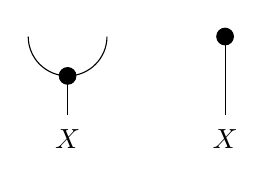
\begin{tikzpicture}
                \draw[fill = black] (0, 0) circle (3pt);
                \draw (-0.5, 0.5) arc (180:360:0.5);
                \draw (0, 0) -- (0, -0.5);
                \node at (0, -0.8) {$X$};
                \draw[fill = black] (2, 0.5) circle (3pt);
                \draw (2, 0.5) -- (2, -0.5);
                \node at (2, -0.8) {$X$};
            \end{tikzpicture}
        \end{gather*}
        From here on, graphical calculus will be adopted.
    \end{notation}

    \begin{remark}[Strictness]
        Depending on the strictness of the monoidal structure, the above coherence conditions can be weakened. If $\symbfsf{M}$ is strict monoidal, the conditions on $\symbf{1}$ hold automatically. Moreover, in this case, \cref{prob:delete_coherence} follows from \cref{prob:copy_coherence}.
    \end{remark}

    \begin{example}
        Every Cartesian category is Markov in a unique way.
    \end{example}

    \newdef{Deterministic morphism}{\index{deterministic}
        A morphism $f:X\rightarrow Y$ in a Markov category that satisfies
        \begin{gather}
            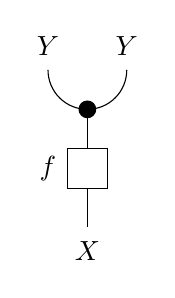
\begin{tikzpicture}[baseline={(0, -0.35)}]
                \node at (-0.5, 0.8) {$Y$};
                \node at (0.5, 0.8) {$Y$};
                \draw[fill = black] (0, 0) circle (3pt);
                \draw (-0.5, 0.5) arc (180:360:0.5);
                \draw (0, 0) -- (0, -1.5);
                \draw[fill = white] (-0.25, -0.5) rectangle (0.25, -1);
                \node at (-0.5, -0.75) {$f$};
                \node at (0, -1.8) {$X$};
            \end{tikzpicture}
            \qquad=\qquad
            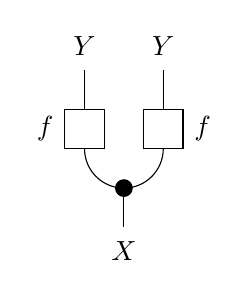
\begin{tikzpicture}[baseline={(0, -0.35)}]
                \node at (-0.5, 0.8) {$Y$};
                \node at (0.5, 0.8) {$Y$};
                \draw (-0.5, 0.5) -- (-0.5, -0.5);
                \draw (0.5, 0.5) -- (0.5, -0.5);
                \draw[fill = white] (-0.75, 0) rectangle (-0.25, -0.5);
                \node at (-1, -0.25) {$f$};
                \draw[fill = white] (0.25, 0) rectangle (0.75, -0.5);
                \node at (1, -0.25) {$f$};
                \draw[fill = black] (0, -1) circle (3pt);
                \draw (-0.5, -0.5) arc (180:360:0.5);
                \draw (0, -1) -- (0, -1.5);
                \node at (0, -1.8) {$X$};
            \end{tikzpicture}\,.
        \end{gather}
        The name stems from the following intuition: If the morphism would be a random transformation of the input, the two applications on the right-hand side might act differently and, hence, the result would not coincide with the two (identical) copies on the left-hand side.
    }

    \newdef{Causal morphism}{\index{causality}
        If the monoidal unit is not required to be terminal, and only coherence conditions~\eqref{prob:tensor_delete} and~\eqref{prob:unit_delete} are required, the resulting structure is sometimes called a \textbf{CD}-category (CD stands for copy and discard). A morphism $f$ in a CD-category is said to be causal or \textbf{terminal} if
        \begin{gather}
            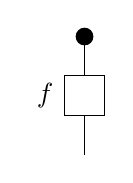
\begin{tikzpicture}[baseline={(0, -0.85)}]
                \draw[fill = black] (0, 0) circle (3pt);
                \draw (0, 0) -- (0, -1.5);
                \draw[fill = white] (-0.25, -0.5) rectangle (0.25, -1);
                \node at (-0.5, -0.75) {$f$};
            \end{tikzpicture}
            \qquad=\qquad
            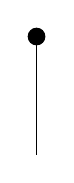
\begin{tikzpicture}[baseline={(0, -0.85)}]
                \draw[fill = black] (0, 0) circle (3pt);
                \draw (0, 0) -- (0, -1.5);
            \end{tikzpicture}\,.
        \end{gather}
        It follows that a Markov category is a CD-category in which all morphisms are causal.
    }

    By generalizing the situation of the Giry monad, distributions in a Markov category can be defined.
    \newdef{Distribution}{\index{distribution}
        Consider a Markov category $(\symbfsf{M},\otimes,\symbf{1})$. A distribution $\psi$ on an object $X\in\ob{M}$ is a global element $\psi:\symbf{1}\rightarrow X$. Graphically this is depicted as follows:
        \begin{gather}
            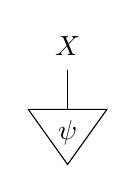
\begin{tikzpicture}[baseline={(0, -0.5)}]
                \node at (0, 0.3) {$X$};
                \draw (0, 0) -- (0, -0.5);
                \draw (-0.5, -0.5) -- (0.5, -0.5) -- (0, -1.2) -- cycle;
                \node at (0, -0.8) {$\psi$};
            \end{tikzpicture}
        \end{gather}
    }
    The category $\symbfsf{Stoch}$, the motivating example of Markov categories, is clearly not Cartesian. If it were, there would be a bijection between joint distributions $\symbf{1}\rightarrow X\otimes Y$ and their marginals $\symbf{1}\rightarrow X$ and $\symbf{1}\rightarrow Y$. However, it is well known that, in general, probability distributions are not uniquely determined by their marginals (cf.~\cref{section:copulas}).

    To take care of countable samples and asymptotic behaviour, it is necessary to extend the monoidal structure to sequences.
    \newdef{Infinite tensor product}{\index{tensor product!infinite}\index{Kolmogorov!product}
        Consider a Markov category $\symbfsf{M}$. For every two finite subsets $A\subseteq B\subset\mathbb{N}$, one obtains a morphism
        \begin{gather}
            \bigotimes_{i\in B}X_i\rightarrow\bigotimes_{j\in A}X_j
        \end{gather}
        by applying the deletion morphism to all objects $X_k$ for $k\in B\backslash A$. The infinite tensor product $\bigotimes_{n\in\mathbb{N}}X_n$ is defined as the inverse/filtered limit of this diagram if
        \begin{enumerate}
            \item it exists, and
            \item is preserved by all $-\otimes Y$ for $Y\in\ob{M}$.
        \end{enumerate}
        If all projection morphisms are deterministic, it is called a \textbf{Kolmogorov product}.
    }